% ============================================================================
\section{Results}\label{sec:results}
% ============================================================================

\subsection{Base case}\label{sec:base}

Table~\ref{tab:base} reports test-set averages over the 100 episodes and Figure~\ref{fig:components} decomposes the costs. Tuning selected order-up-to levels at the 0.95 quantile with daily delivery for BSP and BSP-EW, UL$_\lambda$ with $\lambda=1$, $\alpha=0.95$, $\beta=0.9$, quantile level $\alpha^\star=\alphaQBase$ for LA-Quantile, levels $(0.9,0.8)$ for LA-Quantile2 and budget $\Gamma=\gammaRobBase$ for LA-Robust.

\begin{table}[H]
\centering\footnotesize
\caption{Base case: mean cost per 21-day test episode and its components, fill rate, waste rate (expired units per delivered unit) and store visits per day (100 episodes).}\label{tab:base}
\setlength{\tabcolsep}{4pt}
\resizebox{\textwidth}{!}{\begin{tabular}{lrrrrrrrr}
\toprule
Policy & Total cost (SD) & Routing & Holding & Waste & Lost sales & Fill rate (\%) & Waste rate (\%) & Visits/day \\
\midrule
BSP & 10,472 (2,012) & 4,293 & 2,927 & 475 & 2,777 & 96.5 & 2.55 & 9.5 \\
BSP-EW & 10,515 (1,989) & 4,311 & 2,973 & 478 & 2,752 & 96.5 & 2.57 & 9.6 \\
UL$_\lambda$ & 10,452 (2,061) & 4,240 & 2,935 & 491 & 2,784 & 96.5 & 2.64 & 9.2 \\
LA-Mean & 18,670 (2,772) & 3,935 & 805 & 30 & 13,900 & 81.6 & 0.20 & 9.7 \\
LA-Quantile & 11,768 (2,273) & 3,538 & 3,868 & 1,098 & 3,264 & 95.8 & 5.44 & 7.9 \\
LA-Robust & 11,451 (2,150) & 3,740 & 3,712 & 887 & 3,113 & 96.0 & 4.49 & 8.6 \\
ScenPO-SS & 11,527 (1,732) & 3,419 & 3,832 & 1,063 & 3,213 & 95.9 & 5.35 & 7.7 \\
LA-DFL & 11,085 (2,187) & 3,820 & 2,995 & 532 & 3,738 & 95.2 & 2.76 & 8.9 \\
PI & 5,298 (2,204) & 4,133 & 97 & 0 & 1,068 & 98.8 & 0.00 & 9.9 \\
\bottomrule
\end{tabular}
}
\end{table}

\begin{figure}[H]
\centering
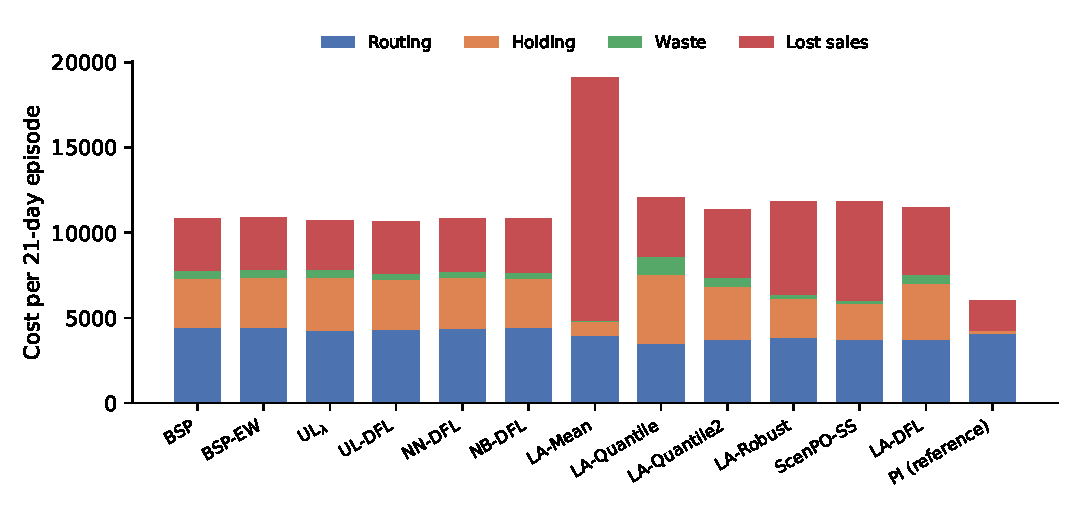
\includegraphics[width=0.85\textwidth]{fig_components.pdf}
\caption{Cost composition of each policy in the base case.}\label{fig:components}
\end{figure}

Four observations stand out. First, uncertainty is expensive: with perfect demand information the same lookahead costs \costPIBase{}, about half of the best implementable policy, almost entirely because lost sales and holding vanish. Second, point forecasts are a poor input for perishable replenishment. LA-Mean plans to sell exactly the expected demand and loses \lostLAMeanBase{} per episode in lost sales (fill rate \fillLAMeanBase\%), as Proposition~\ref{prop:marginal} suggests when $p_u$ is four times $p_s$. Third, among the policies without learning, the three stock-age-based inventory rules are the cheapest: UL$_\lambda$, BSP and BSP-EW cost between \costULBase{} and \costBSPEWBase{} with a fill rate of \fillULBase\% and a waste rate of about 2.5\%. With daily review, little of the current stock is at risk of expiring before it is sold, so the waste correction of BSP-EW rarely changes an order.

Fourth, integration with routing does reduce travel but loses more on the inventory side. The uncertainty-aware lookahead policies visit 7.7--9.0 stores per day instead of 9.2--9.6 and save about 500--1,000 in routing, but LA-Quantile and ScenPO-SS hold 26--37\% more stock than the rules and waste about twice as much (waste rates \wasteScenPOBase\% and \wasteLAQBase\%), while LA-Robust avoids the waste at the price of a fill rate of \fillLARobBase\%. A deterministic plan that covers two or three days with quantile targets stacks a safety buffer on every covered day, even though the next day's re-planning will correct any shortfall. LA-Quantile2, which keeps the 0.9 quantile only for the implemented day and plans later days at the 0.8 quantile, halves the waste rate of LA-Quantile (\wasteLAQTwoBase\% vs.\ \wasteLAQBase\%) and costs 5.7\% less; the scenario model reduces lost sales but, because its single plan must work for all scenarios, it also covers several days generously.

\begin{table}[H]
\centering\footnotesize
\caption{Paired episode-level comparisons of UL-DFL with every other policy (base case, 100 episodes). Negative differences favour UL-DFL. Holm adjustment over the five prespecified primary comparisons of UL-DFL.}\label{tab:testsul}
\setlength{\tabcolsep}{4pt}
\resizebox{\textwidth}{!}{\begin{tabular}{lrrrrrrr}
\toprule
Comparison & Mean diff. & 95\% bootstrap CI & Rel. (\%) & Wins (\%) & $p$ ($t$) & $p$ (Wilcoxon) & Holm $p$ \\
\midrule
UL-DFL $-$ BSP & -213.8 & [-265.8, -160.5] & -2.0 & 80 & $<$0.001 & $<$0.001 & -- \\
UL-DFL $-$ BSP-EW & -236.1 & [-289.0, -182.5] & -2.2 & 80 & $<$0.001 & $<$0.001 & $<$0.001 \\
UL-DFL $-$ UL$_\lambda$ & -107.4 & [-153.1, -60.5] & -1.1 & 67 & $<$0.001 & $<$0.001 & $<$0.001 \\
UL-DFL $-$ NN-DFL & -201.3 & [-254.4, -149.7] & -1.7 & 78 & $<$0.001 & $<$0.001 & -- \\
UL-DFL $-$ NB-DFL & -180.5 & [-225.4, -136.3] & -1.6 & 80 & $<$0.001 & $<$0.001 & -- \\
UL-DFL $-$ LA-Mean & -8,465.5 & [-8,764.1, -8,175.6] & -44.4 & 100 & $<$0.001 & $<$0.001 & -- \\
UL-DFL $-$ LA-Quantile & -1,434.2 & [-1,585.6, -1,278.2] & -11.8 & 98 & $<$0.001 & $<$0.001 & -- \\
UL-DFL $-$ LA-Quantile2 & -752.9 & [-872.7, -629.9] & -6.3 & 92 & $<$0.001 & $<$0.001 & $<$0.001 \\
UL-DFL $-$ LA-Robust & -1,193.9 & [-1,313.2, -1,076.2] & -10.0 & 99 & $<$0.001 & $<$0.001 & -- \\
UL-DFL $-$ ScenPO-SS & -1,199.2 & [-1,342.1, -1,056.2] & -10.3 & 95 & $<$0.001 & $<$0.001 & $<$0.001 \\
UL-DFL $-$ LA-DFL & -819.9 & [-958.9, -684.2] & -6.7 & 95 & $<$0.001 & $<$0.001 & $<$0.001 \\
UL-DFL $-$ PI & 4,630.0 & [4,454.8, 4,800.8] & 87.0 & 0 & $<$0.001 & $<$0.001 & -- \\
\bottomrule
\end{tabular}
}
\end{table}

UL-DFL is the cheapest implementable policy (Table~\ref{tab:testsul}). It costs \ULabsrelULBase\% less than the tuned UL$_\lambda$ from which it starts (95\% CI \ULciULBase{}, lower in \ULwinULBase\% of the episodes), \ULabsrelBSPEWBase\% less than BSP-EW, \ULabsrelScenPOBase\% less than ScenPO-SS, \ULabsrelLAQTwoBase\% less than LA-Quantile2 and \ULabsrelDFLBase\% less than LA-DFL; all five primary comparisons are significant after Holm adjustment ($p<0.001$). The gain over UL$_\lambda$ is a waste reduction: at the same fill rate (\fillULDFLBase\%) and almost the same lost-sales cost, UL-DFL lowers the waste rate from \wasteULBase\% to \wasteULDFLBase\%, i.e.\ it throws away a fifth fewer units, while holding and routing costs rise by at most 0.5\%.

\begin{table}[H]
\centering\footnotesize
\caption{Paired episode-level comparisons of LA-DFL with every other policy (base case, 100 episodes). Negative differences favour LA-DFL. Holm adjustment over the five prespecified primary comparisons of LA-DFL.}\label{tab:tests}
\setlength{\tabcolsep}{4pt}
\resizebox{\textwidth}{!}{\begin{tabular}{lrrrrrrr}
\toprule
Comparison & Mean diff. & 95\% bootstrap CI & Rel. (\%) & Wins (\%) & $p$ ($t$) & $p$ (Wilcoxon) & Holm $p$ \\
\midrule
LA-DFL $-$ BSP & 696.8 & [551.8, 844.2] & 6.4 & 18 & $<$0.001 & $<$0.001 & -- \\
LA-DFL $-$ BSP-EW & 662.5 & [517.0, 810.7] & 6.0 & 21 & $<$0.001 & $<$0.001 & $<$0.001 \\
LA-DFL $-$ UL$_\lambda$ & 749.0 & [606.5, 891.8] & 7.0 & 14 & $<$0.001 & $<$0.001 & $<$0.001 \\
LA-DFL $-$ UL-DFL & 839.7 & [705.7, 972.4] & 7.8 & 6 & $<$0.001 & $<$0.001 & -- \\
LA-DFL $-$ NN-DFL & 677.0 & [556.9, 797.0] & 6.2 & 13 & $<$0.001 & $<$0.001 & -- \\
LA-DFL $-$ LA-Mean & -7,822.9 & [-8,167.1, -7,477.1] & -40.4 & 100 & $<$0.001 & $<$0.001 & -- \\
LA-DFL $-$ LA-Quantile & -573.7 & [-683.7, -465.2] & -4.9 & 84 & $<$0.001 & $<$0.001 & $<$0.001 \\
LA-DFL $-$ LA-Quantile2 & 115.0 & [41.2, 190.6] & 1.0 & 41 & 0.004 & 0.015 & -- \\
LA-DFL $-$ LA-Robust & -400.0 & [-542.4, -255.7] & -3.4 & 70 & $<$0.001 & $<$0.001 & $<$0.001 \\
LA-DFL $-$ ScenPO-SS & -154.5 & [-365.6, 67.9] & -1.6 & 59 & 0.167 & 0.124 & 0.167 \\
LA-DFL $-$ PI & 5,789.9 & [5,575.4, 6,009.5] & 110.2 & 0 & $<$0.001 & $<$0.001 & -- \\
\bottomrule
\end{tabular}
}
\end{table}

LA-DFL improves the deterministic lookahead from which it starts (Table~\ref{tab:tests}). It reduces cost by \absrelLAQBase\% relative to LA-Quantile (95\% CI \ciLAQBase{}, lower in \winLAQBase\% of the episodes) and by \absrelLARobBase\% relative to LA-Robust; it is \absrelScenPOBase\% cheaper than ScenPO-SS, which is not significant (Holm-adjusted $p=$ \pholmScenPOBase{}). It does so by halving the waste rate of LA-Quantile (\wasteDFLBase\% vs.\ \wasteLAQBase\%) while accepting somewhat more lost sales. The simple LA-Quantile2, however, is \absrelLAQTwoBase\% cheaper still (CI \ciLAQTwoBase{}): the gain of LA-DFL over LA-Quantile is captured by a day-specific quantile level, which LA-DFL discovered (Section~\ref{sec:dflresults}) but did not improve on. LA-DFL also remains \absrelBSPEWBase\% more expensive than BSP-EW and \absrelULBase\% more expensive than UL$_\lambda$, both significant.

\subsection{What the decision-focused corrections learn}\label{sec:dflresults}

Table~\ref{tab:ulcorrections} summarises the learned corrections of UL-DFL on the delivery decisions it takes in the 100 base-case test episodes (the rule triggers a delivery on 94\% of the store-days; on the others the correction has no effect). The average correction is nearly zero: the tuned 0.95 level is right on average. What the network learns is \emph{when} to deviate from it, along two dimensions that a one-day order-up-to rule cannot see. On promotion days it lowers the level to an implied service level of about 0.89, i.e.\ by about a third of a day of mean demand. Promotions raise the forecast spread, so the 0.95 quantile lies far above the expected demand, and whatever is left when the promotion ends meets regular demand and ages. Over the week it raises the level from Wednesday to Friday (implied levels 0.96--0.97) and lowers it from Saturday to Monday (0.92--0.93): a unit left over before the weekend is sold in the Saturday peak, whereas a unit left over after it meets lower demand for the rest of its shelf life. The age of the stock on hand matters little, because the rule's order quantity already nets out the stock projected to expire. Both corrections reduce the stock that is still on the shelf when demand falls, which is where the waste of the rule arises.

\begin{table}[H]
\centering\footnotesize
\caption{Learned corrections of UL-DFL on the delivery decisions of 100 test episodes (base case): mean correction $\delta_\theta$ of the order-up-to level in units of the forecast scale, implied service level $\Phi(z_{0.95}+\delta_\theta)$, and change of the order-up-to level in days of mean store demand. Stock is measured in days of mean store demand.}\label{tab:ulcorrections}
\resizebox{0.85\textwidth}{!}{\begin{tabular}{lrrrr}
\toprule
Delivery decisions & $n$ & Correction $\delta_\theta$ (SD) & Implied service level & Change of $S$ (days) \\
\midrule
all delivery decisions & 18,952 & -0.13 (0.30) & 0.940 & -0.07 \\
no promotion & 16,404 & -0.08 (0.27) & 0.947 & -0.03 \\
promotion & 2,548 & -0.48 (0.27) & 0.890 & -0.37 \\
Mon & 2,715 & -0.31 (0.20) & 0.921 & -0.14 \\
Tue & 2,653 & -0.14 (0.22) & 0.941 & -0.07 \\
Wed & 2,745 & +0.01 (0.20) & 0.958 & -0.01 \\
Thu & 2,725 & +0.21 (0.23) & 0.972 & +0.09 \\
Fri & 2,755 & +0.06 (0.23) & 0.961 & +0.02 \\
Sat & 2,854 & -0.39 (0.20) & 0.908 & -0.23 \\
Sun & 2,505 & -0.35 (0.21) & 0.914 & -0.17 \\
stock <0.25 d & 4,450 & -0.09 (0.30) & 0.945 & -0.05 \\
stock 0.25-0.5 d & 2,595 & -0.12 (0.29) & 0.941 & -0.06 \\
stock >0.5 d & 11,907 & -0.15 (0.31) & 0.937 & -0.08 \\
no expiring units & 13,299 & -0.11 (0.30) & 0.942 & -0.06 \\
units expiring today & 5,653 & -0.19 (0.30) & 0.933 & -0.10 \\
\bottomrule
\end{tabular}
}
\end{table}

Table~\ref{tab:corrections} reports the corrections of LA-DFL on the decision states of 20 test episodes. Here the dominant pattern is temporal within the plan. For the implemented day the network keeps the target at about the 0.91 quantile, essentially the tuned LA-Quantile level, but it lowers the targets of the second and third lookahead days to about the 0.80 and 0.77 quantiles. In inventory terms, the network has learned that only today's shortfall is irreversible: tomorrow's planned demand will be re-planned with tomorrow's stock and forecast, so a full safety buffer on that day mostly turns into carried stock and, with a three-day shelf life, into waste. This is precisely the recourse that a deterministic lookahead ignores and that Proposition~\ref{prop:dfl} lets the gradient account for. Context-specific corrections are small: targets are lowered somewhat more on promotion days and slightly less when the store holds more or older stock. The day-specific levels learned by LA-DFL are those that the tuning of LA-Quantile2 selects, $(0.9,0.8)$, which explains why the two policies perform alike.

\begin{table}[H]
\centering\footnotesize
\caption{Learned corrections of LA-DFL on the decision states of 20 test episodes (base case): mean correction $\delta_\theta$ in forecast-scale units, implied quantile level of the planning target, and target relative to the mean forecast. $k$ is the lookahead offset; stock is measured in days of mean store demand.}\label{tab:corrections}
\resizebox{0.85\textwidth}{!}{\begin{tabular}{lrrrr}
\toprule
Targets & $n$ & Correction $\delta_\theta$ (SD) & Implied quantile level & Target / mean forecast \\
\midrule
all & 12,600 & -0.37 (0.38) & 0.826 & 1.46 \\
k=0 & 4,200 & +0.12 (0.15) & 0.910 & 1.67 \\
k=1 & 4,200 & -0.53 (0.15) & 0.804 & 1.38 \\
k=2 & 4,200 & -0.69 (0.17) & 0.765 & 1.31 \\
no promotion & 11,078 & -0.36 (0.39) & 0.828 & 1.45 \\
promotion & 1,522 & -0.47 (0.32) & 0.818 & 1.53 \\
stock <0.25 d & 2,694 & -0.42 (0.39) & 0.816 & 1.43 \\
stock 0.25-0.75 d & 4,059 & -0.40 (0.38) & 0.821 & 1.45 \\
stock >0.75 d & 5,847 & -0.33 (0.38) & 0.835 & 1.48 \\
no expiring units & 8,088 & -0.39 (0.38) & 0.822 & 1.45 \\
units expiring today & 4,512 & -0.33 (0.38) & 0.834 & 1.48 \\
\bottomrule
\end{tabular}
}
\end{table}

For both learners the closed-loop validation cost improved during the first three to five epochs and deteriorated afterwards (Figure~\ref{fig:dfltraining}), which is why model selection on closed-loop validation cost is part of the method. The result does not depend on a lucky seed (Table~\ref{tab:seeds}): the three UL-DFL networks are 0.8--0.9\% cheaper than UL$_\lambda$ on the base-case test set, and the three LA-DFL networks 3.5--4.7\% cheaper than LA-Quantile.

\begin{figure}[H]
\centering
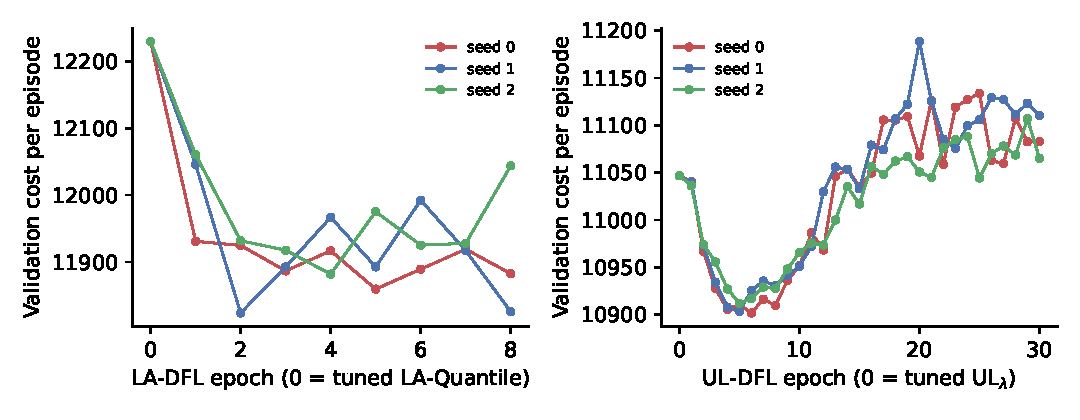
\includegraphics[width=0.9\textwidth]{fig_dfl_training.pdf}
\caption{Closed-loop validation cost by training epoch and seed (base case). Left: LA-DFL, epoch 0 is the tuned LA-Quantile policy. Right: UL-DFL, epoch 0 is the tuned UL$_\lambda$ rule.}\label{fig:dfltraining}
\end{figure}

\begin{table}[H]
\centering\footnotesize
\caption{Test-cost difference (\%) of each trained network relative to the policy it starts from, by seed; ``selected'' is the network chosen on validation cost.}\label{tab:seeds}
\begin{tabular}{llrrrr}
\toprule
Setting & Comparison & Selected (\%) & Seed 0 & Seed 1 & Seed 2 \\
\midrule
Base (fresh test) & UL-DFL vs UL$_\lambda$ & -1.05 & -1.05 & -1.02 & -0.98 \\
Base (fresh test) & NN-DFL vs UL$_\lambda$ & +0.75 & +0.49 & +0.86 & +0.75 \\
Base (fresh test) & NB-DFL vs UL$_\lambda$ & +0.57 & +0.52 & +0.57 & +0.89 \\
Base & UL-DFL vs UL$_\lambda$ & -0.81 & -0.81 & -0.75 & -0.93 \\
Base & NN-DFL vs UL$_\lambda$ & +1.25 & +1.26 & +1.18 & +1.25 \\
Base & NB-DFL vs UL$_\lambda$ & +1.00 & +0.97 & +1.00 & +1.26 \\
Base & LA-DFL vs LA-Quantile & -4.86 & -3.71 & -4.86 & -3.59 \\
Clustered & UL-DFL vs UL$_\lambda$ & -1.21 & -1.21 & -1.17 & -1.15 \\
Clustered & NN-DFL vs UL$_\lambda$ & +0.02 & +0.08 & +0.02 & +0.16 \\
Clustered & NB-DFL vs UL$_\lambda$ & -0.27 & -0.21 & -0.27 & +0.18 \\
Mixed & UL-DFL vs UL$_\lambda$ & -1.02 & -1.02 & -1.02 & -0.95 \\
Mixed & NN-DFL vs UL$_\lambda$ & +0.28 & +0.25 & +0.04 & +0.28 \\
Mixed & NB-DFL vs UL$_\lambda$ & -0.03 & +0.01 & -0.03 & +0.29 \\
$m=2$ & UL-DFL vs UL$_\lambda$ & -1.12 & -1.11 & -1.00 & -1.12 \\
$m=2$ & NN-DFL vs UL$_\lambda$ & -0.49 & -0.61 & -0.55 & -0.49 \\
$m=2$ & NB-DFL vs UL$_\lambda$ & -0.42 & -0.34 & -0.21 & -0.42 \\
$m=4$ & UL-DFL vs UL$_\lambda$ & -0.30 & -0.30 & -0.27 & -0.19 \\
$m=4$ & NN-DFL vs UL$_\lambda$ & +2.49 & +2.40 & +2.47 & +2.42 \\
$m=4$ & NB-DFL vs UL$_\lambda$ & +1.66 & +1.66 & +2.09 & +1.96 \\
$p_u=10$ & UL-DFL vs UL$_\lambda$ & -0.96 & -0.92 & -0.96 & -0.89 \\
$p_u=10$ & NN-DFL vs UL$_\lambda$ & +1.15 & +1.25 & +1.25 & +1.15 \\
$p_u=10$ & NB-DFL vs UL$_\lambda$ & +0.84 & +0.88 & +0.84 & +0.90 \\
$p_u=40$ & UL-DFL vs UL$_\lambda$ & -0.84 & -0.89 & -0.84 & -0.88 \\
$p_u=40$ & NN-DFL vs UL$_\lambda$ & +0.68 & +0.68 & +0.63 & +1.08 \\
$p_u=40$ & NB-DFL vs UL$_\lambda$ & +1.30 & +1.59 & +1.30 & +1.55 \\
$\rho=1.10$ & UL-DFL vs UL$_\lambda$ & -0.81 & -0.81 & -0.76 & -0.76 \\
$\rho=1.10$ & NN-DFL vs UL$_\lambda$ & +0.74 & +0.47 & +0.74 & +0.79 \\
$\rho=1.10$ & NB-DFL vs UL$_\lambda$ & +0.65 & +0.66 & +0.65 & +0.76 \\
$\rho=1.60$ & UL-DFL vs UL$_\lambda$ & -0.30 & -0.31 & -0.30 & -0.35 \\
$\rho=1.60$ & NN-DFL vs UL$_\lambda$ & +1.54 & +1.66 & +1.75 & +1.54 \\
$\rho=1.60$ & NB-DFL vs UL$_\lambda$ & +1.32 & +1.33 & +1.32 & +1.30 \\
High var. & UL-DFL vs UL$_\lambda$ & -0.00 & +0.04 & -0.00 & -0.18 \\
High var. & NN-DFL vs UL$_\lambda$ & +0.86 & +0.74 & +0.92 & +0.86 \\
High var. & NB-DFL vs UL$_\lambda$ & +1.30 & +1.39 & +1.30 & +1.56 \\
$c^{\mathrm{r}}=3$ & UL-DFL vs UL$_\lambda$ & -0.81 & -0.93 & -0.81 & -0.73 \\
$c^{\mathrm{r}}=3$ & NN-DFL vs UL$_\lambda$ & +4.56 & +4.69 & +4.65 & +4.56 \\
$c^{\mathrm{r}}=3$ & NB-DFL vs UL$_\lambda$ & +4.50 & +4.30 & +4.50 & +4.39 \\
30\% LIFO & UL-DFL vs UL$_\lambda$ & -0.80 & -0.80 & -0.75 & -0.82 \\
30\% LIFO & NN-DFL vs UL$_\lambda$ & +1.75 & +1.67 & +2.02 & +1.75 \\
30\% LIFO & NB-DFL vs UL$_\lambda$ & +1.43 & +1.39 & +1.43 & +1.56 \\
30\% LIFO & LA-DFL vs LA-Quantile & -4.94 & -4.43 & -4.94 & -3.43 \\
Real data & UL-DFL vs UL$_\lambda$ & +0.62 & +0.51 & +0.09 & +0.62 \\
Real data & NN-DFL vs UL$_\lambda$ & +1.44 & +1.78 & +1.44 & +1.60 \\
Real data & NB-DFL vs UL$_\lambda$ & +1.13 & +1.13 & +1.37 & +1.70 \\
\bottomrule
\end{tabular}

\end{table}

\subsection{Can re-tuning the rule reproduce UL-DFL?}\label{sec:frontier}

A natural objection is that UL-DFL merely finds better values of the rule's parameters than the tuning grid of Section~\ref{sec:design}. Figure~\ref{fig:frontier} places UL-DFL in the waste--service plane together with 124 parameterisations of the rules, all evaluated on the base-case test episodes: UL$_\lambda$ with $\lambda=1$, ten service levels $\alpha$ between 0.85 and 0.99 and eight trigger levels $\beta$ between 0.5 and 0.99, UL$_\lambda$ with $\lambda\in\{2,3\}$ on the original grid, and daily BSP and BSP-EW at the same ten service levels. No parameterisation serves at least UL-DFL's fill rate (96.2\%) with no more waste: at that fill rate the least waste any rule achieves is 2.48\% of the delivered units, against 1.98\% for UL-DFL. The learned corrections move the policy beyond the waste--service frontier of the rules, which no choice of a single service level and trigger can do.

In total cost the comparison is closer. The cheapest of the 124 rules in hindsight---selected on the test episodes themselves, an advantage UL-DFL does not have---is UL$_\lambda$ with $\alpha=0.96$ and $\beta=0.8$. It costs 10,715 per episode, the same as UL-DFL (difference $-0.05\%$, 95\% CI $[-59, 46]$), but it gets there differently: its lower trigger saves routing (4,168 vs.\ 4,337), and it wastes 2.80\% of the delivered units, 41\% more than UL-DFL. Part of the 0.8\% cost advantage of UL-DFL over the tuned rule therefore reflects the resolution of the tuning grid; the waste reduction at a given service level does not. The real-data case gives the same picture: no rule parameterisation reaches UL-DFL's fill rate (93.8\%) with its waste rate (2.96\%; the least any rule achieves at that fill rate is 3.15\%), and the best rule in hindsight ($\alpha=0.96$, $\beta=0.85$) matches its cost ($+0.02\%$ for UL-DFL, 95\% CI $[-50, 78]$) while wasting 23\% more.

\begin{figure}[H]
\centering
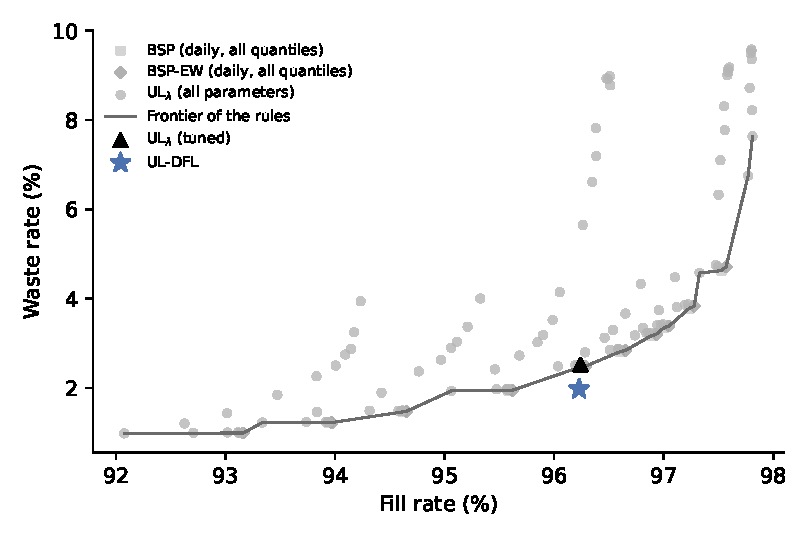
\includegraphics[width=0.62\textwidth]{fig_frontier.pdf}
\caption{Waste rate against fill rate of 124 parameterisations of the rules and of UL-DFL (base case, 100 test episodes). The line connects the rule parameterisations that are not dominated in both measures.}\label{fig:frontier}
\end{figure}

\subsection{Does the learner need the rule?}\label{sec:nndfl}

The converse question is whether the rule contributes anything once a network is trained on realised cost. NN-DFL answers it: it has the same inputs, differentiable simulation, loss, seeds and model selection as UL-DFL, but outputs the delivery directly, without the visit trigger and order-up-to structure of UL$_\lambda$. In the base case it costs \costNNDFLBase{} per episode, \ULabsrelNNDFLBase\% more than UL-DFL (95\% CI of UL-DFL minus NN-DFL \ULciNNDFLBase{}) and more than the tuned UL$_\lambda$ it would replace. It does learn to waste little (waste rate \wasteNNDFLBase\%), but it loses more sales and, lacking a trigger, visits slightly more stores (\visitsNNDFLBase{} per day against \visitsULDFLBase{}). Across the thirteen configurations UL-DFL is significantly cheaper than NN-DFL in twelve, by 0.8--4.9\% (Table~\ref{tab:uldfldiffs}). The gap is largest with expensive routing, where the trigger of UL-DFL cuts store visits to \visitsULDFLRouteThree{} per day while NN-DFL keeps visiting \visitsNNDFLRouteThree{}, and the two tie with a two-day shelf life, where frequent small deliveries suit the short shelf life. NN-DFL is more expensive than UL$_\lambda$ itself in eleven of the thirteen configurations (Table~\ref{tab:seeds}). These comparisons are secondary, because the ablation was added after the primary hypotheses were fixed, but they are consistent: with the same network and learning signal, the gain comes from placing the learner on the rule.

\subsection{Sensitivity analysis}\label{sec:sensitivity}

Table~\ref{tab:sensitivity} reports test costs across the configurations, and Tables~\ref{tab:uldfldiffs} and~\ref{tab:dfldiffs} the paired differences of the two learned policies. \SensitivityText

\begin{table}[H]
\centering\footnotesize
\caption{Mean test cost per episode by configuration (one factor changed at a time; bold: lowest implementable policy), and fill rates of selected policies.}\label{tab:sensitivity}
\setlength{\tabcolsep}{4pt}
\resizebox{\textwidth}{!}{\begin{tabular}{lrrrrrrrrrrrrr}
\toprule
Policy & Base & Clustered & Mixed & $m=2$ & $m=4$ & $p_u=10$ & $p_u=40$ & $\rho=1.10$ & $\rho=1.60$ & High var. & $c^{\mathrm{r}}=3$ & 30\% LIFO & Real data \\
\midrule
BSP & 10,851 & 8,266 & 10,206 & 12,607 & 10,490 & 9,056 & 13,480 & 12,221 & 9,868 & 15,011 & 19,633 & 11,208 & 13,068 \\
BSP-EW & 10,885 & 8,289 & 10,235 & 12,633 & 10,490 & 9,082 & 13,496 & 12,227 & 9,922 & 15,089 & 19,704 & 11,256 & 13,090 \\
UL$_\lambda$ & 10,799 & 8,274 & 10,199 & 12,599 & 10,339 & 8,956 & 13,374 & 12,152 & 9,798 & 14,885 & 18,856 & 11,141 & 13,027 \\
UL-DFL & \textbf{10,708} & \textbf{8,168} & \textbf{10,090} & 12,487 & \textbf{10,324} & \textbf{8,867} & \textbf{13,251} & \textbf{12,063} & \textbf{9,755} & \textbf{14,845} & 18,700 & \textbf{11,057} & \textbf{12,951} \\
NN-DFL & 10,871 & 8,263 & 10,221 & \textbf{12,483} & 10,534 & 9,052 & 13,396 & 12,179 & 9,892 & 14,974 & 19,645 & 11,253 & 13,093 \\
LA-Mean & 19,371 & 17,051 & 18,362 & 19,769 & 19,350 & 12,074 & 33,960 & 19,362 & 19,407 & 25,609 & 24,289 & 19,400 & 21,030 \\
LA-Quantile & 12,122 & 9,735 & 11,520 & 13,954 & 11,289 & 9,314 & 15,490 & 13,327 & 10,405 & 16,398 & 19,157 & 12,574 & 14,478 \\
LA-Quantile2 & 11,433 & 9,110 & 10,830 & 13,553 & 10,977 & 9,136 & 15,436 & 13,047 & 10,071 & 15,631 & 18,630 & 11,787 & 14,185 \\
LA-Robust & 11,948 & 9,545 & 11,209 & 13,622 & 11,221 & 9,173 & 15,295 & 13,291 & 10,184 & 15,851 & 18,983 & 12,110 & 14,560 \\
ScenPO-SS & 11,702 & 9,544 & 11,315 & 13,179 & 11,051 & 9,393 & 14,501 & 12,512 & 10,997 & 16,218 & \textbf{18,197} & 12,162 & 13,776 \\
LA-DFL & 11,548 & 9,294 & 11,089 & 14,295 & 11,015 & 9,258 & 15,498 & 13,260 & 10,146 & 16,101 & 19,058 & 11,974 & 14,333 \\
\midrule
PI (reference) & 5,758 & 3,352 & 5,180 & 6,121 & 5,752 & 5,005 & 7,260 & 7,678 & 4,728 & 7,097 & 13,589 & 5,758 & 7,329 \\
\midrule
Fill rate (\%), UL-DFL & 96.2 & 96.2 & 96.2 & 94.8 & 96.6 & 94.6 & 97.1 & 94.8 & 97.1 & 93.1 & 95.9 & 96.2 & 93.8 \\
Fill rate (\%), LA-DFL & 95.1 & 95.2 & 95.1 & 93.1 & 95.4 & 93.4 & 95.8 & 92.8 & 96.3 & 91.9 & 94.9 & 94.9 & 92.1 \\
Fill rate (\%), ScenPO-SS & 95.6 & 96.1 & 95.7 & 95.0 & 95.7 & 92.0 & 97.1 & 93.8 & 96.0 & 92.0 & 94.2 & 95.5 & 93.1 \\
Fill rate (\%), LA-Quantile & 95.7 & 96.2 & 96.1 & 91.2 & 95.9 & 92.7 & 95.8 & 91.6 & 96.3 & 89.1 & 93.0 & 95.6 & 92.8 \\
Fill rate (\%), BSP-EW & 96.3 & 96.3 & 96.3 & 94.5 & 96.3 & 94.7 & 97.0 & 94.5 & 97.4 & 93.8 & 96.3 & 96.2 & 93.8 \\
\bottomrule
\end{tabular}
}
\end{table}

\begin{table}[H]
\centering\footnotesize
\caption{Paired cost difference of UL-DFL relative to each comparator, in percent of the comparator's cost, by configuration. Bold: 95\% paired bootstrap interval excludes zero.}\label{tab:uldfldiffs}
\resizebox{\textwidth}{!}{\begin{tabular}{lrrrrrrrrrrrrr}
\toprule
UL-DFL & Base & Clustered & Mixed & $m=2$ & $m=4$ & $p_u=10$ & $p_u=40$ & $\rho=1.10$ & $\rho=1.60$ & High var. & $c^{\mathrm{r}}=3$ & 30\% LIFO & Real data \\
\midrule
vs UL$_\lambda$ & \textbf{-0.8} & \textbf{-1.2} & \textbf{-1.0} & \textbf{-1.1} & -0.3 & \textbf{-1.0} & \textbf{-0.8} & \textbf{-0.8} & -0.3 & -0.0 & \textbf{-0.8} & \textbf{-0.8} & \textbf{+0.6} \\
vs BSP-EW & \textbf{-2.2} & \textbf{-1.5} & \textbf{-1.4} & \textbf{-1.8} & \textbf{-2.2} & \textbf{-2.4} & \textbf{-2.2} & \textbf{-1.9} & \textbf{-2.1} & \textbf{-1.8} & \textbf{-5.4} & \textbf{-2.6} & -0.5 \\
vs ScenPO-SS & \textbf{-10.8} & \textbf{-15.9} & \textbf{-13.6} & \textbf{-4.4} & \textbf{-13.4} & \textbf{-9.9} & \textbf{-13.2} & \textbf{-4.7} & \textbf{-19.6} & \textbf{-11.5} & \textbf{-3.4} & \textbf{-9.9} & \textbf{-8.3} \\
vs LA-DFL & \textbf{-7.5} & \textbf{-11.4} & \textbf{-8.5} & \textbf{-12.3} & \textbf{-6.7} & \textbf{-4.1} & \textbf{-14.6} & \textbf{-9.4} & \textbf{-4.1} & \textbf{-7.8} & \textbf{-2.1} & \textbf{-7.9} & \textbf{-9.6} \\
vs LA-Quantile2 & \textbf{-6.6} & \textbf{-9.8} & \textbf{-6.1} & \textbf{-7.6} & \textbf{-6.5} & \textbf{-2.9} & \textbf{-14.3} & \textbf{-7.8} & \textbf{-3.4} & \textbf{-5.0} & +0.1 & \textbf{-6.6} & \textbf{-8.4} \\
vs NN-DFL & \textbf{-2.0} & \textbf{-1.1} & \textbf{-1.2} & \textbf{-0.6} & \textbf{-2.7} & \textbf{-2.1} & \textbf{-1.4} & \textbf{-1.5} & \textbf{-1.8} & \textbf{-0.8} & \textbf{-5.1} & \textbf{-2.4} & -0.8 \\
\bottomrule
\end{tabular}
}
\end{table}

\begin{table}[H]
\centering\footnotesize
\caption{Paired cost difference of LA-DFL relative to each comparator, in percent of the comparator's cost, by configuration. Bold: 95\% paired bootstrap interval excludes zero.}\label{tab:dfldiffs}
\resizebox{\textwidth}{!}{\begin{tabular}{lrrrrrrrrrrrrr}
\toprule
LA-DFL & Base & Clustered & Mixed & $m=2$ & $m=4$ & $p_u=10$ & $p_u=40$ & $\rho=1.10$ & $\rho=1.60$ & High var. & $c^{\mathrm{r}}=3$ & 30\% LIFO & Real data \\
\midrule
vs LA-Quantile & \textbf{-4.9} & \textbf{-5.0} & \textbf{-3.9} & \textbf{+2.1} & \textbf{-2.5} & -0.7 & +0.0 & -0.8 & \textbf{-2.4} & \textbf{-1.7} & -0.4 & \textbf{-4.9} & -1.4 \\
vs LA-Quantile2 & \textbf{+1.0} & \textbf{+1.9} & \textbf{+2.8} & \textbf{+5.7} & +0.3 & \textbf{+1.4} & +0.7 & \textbf{+1.8} & +0.8 & \textbf{+3.3} & \textbf{+2.4} & \textbf{+1.5} & +1.5 \\
vs ScenPO-SS & -1.6 & -3.4 & \textbf{-2.4} & \textbf{+7.7} & -0.5 & \textbf{-1.4} & \textbf{+6.4} & \textbf{+5.6} & \textbf{-7.6} & -0.8 & \textbf{+4.8} & -1.9 & \textbf{+4.5} \\
vs LA-Robust & \textbf{-3.4} & \textbf{-2.9} & -1.1 & \textbf{+4.8} & \textbf{-1.8} & \textbf{+0.9} & +1.9 & -0.2 & -0.3 & \textbf{+1.8} & +0.5 & -1.2 & -0.6 \\
vs BSP-EW & \textbf{+6.0} & \textbf{+11.8} & \textbf{+8.1} & \textbf{+12.7} & \textbf{+5.1} & \textbf{+1.9} & \textbf{+15.2} & \textbf{+8.6} & \textbf{+2.2} & \textbf{+6.8} & \textbf{-3.3} & \textbf{+6.2} & \textbf{+10.5} \\
vs UL$_\lambda$ & \textbf{+7.0} & \textbf{+12.1} & \textbf{+8.6} & \textbf{+13.1} & \textbf{+6.6} & \textbf{+3.5} & \textbf{+16.0} & \textbf{+9.2} & \textbf{+3.5} & \textbf{+8.4} & \textbf{+1.3} & \textbf{+7.4} & \textbf{+11.2} \\
\bottomrule
\end{tabular}
}
\end{table}

\begin{figure}[H]
\centering
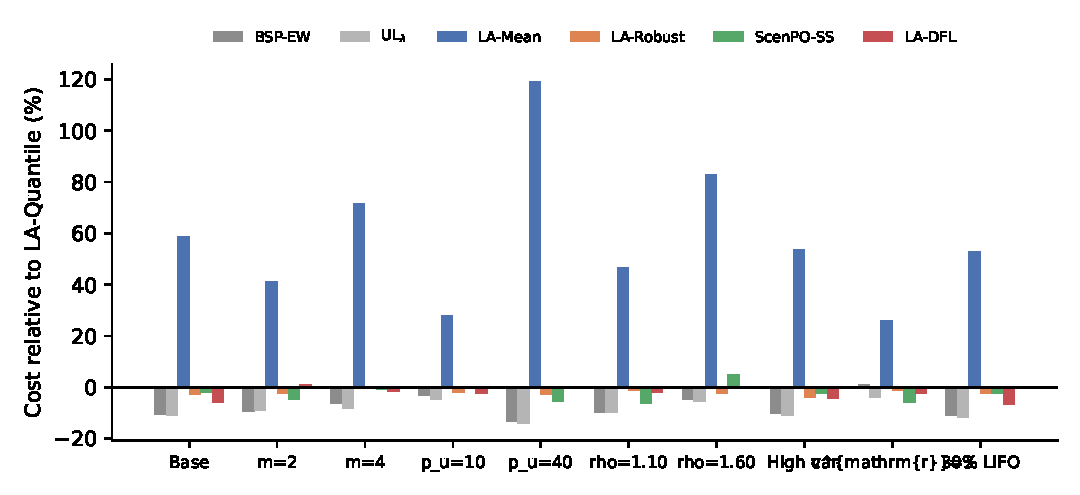
\includegraphics[width=0.95\textwidth]{fig_sensitivity.pdf}
\caption{Cost of selected policies relative to LA-Quantile, by configuration (LA-Mean is omitted for readability).}\label{fig:sensitivity}
\end{figure}

\subsection{Real-data case}\label{sec:realresults}

On observed demand (column ``Real data'' of Tables~\ref{tab:sensitivity} and~\ref{tab:uldfldiffs}) the ranking of the policy families is the same as in the synthetic base case. UL-DFL is the cheapest policy (\costULDFLFresh{} per episode), \ULabsrelULFresh\% below UL$_\lambda$ (95\% CI \ULciULFresh{}, Holm-adjusted $p=\ULpholmULFresh$), \ULabsrelBSPEWFresh\% below BSP-EW and \ULabsrelScenPOFresh\% below ScenPO-SS, the best integrated policy. Without learning, the rules (\costULFresh--\costBSPEWFresh) are again cheaper than every integrated policy, and LA-Mean is again the most expensive. Service is lower than in the synthetic study for all policies (fill rate \fillULFresh\% for UL$_\lambda$), because observed demand is more volatile and its promotion and weekend peaks occasionally exceed the daily fleet capacity.

The saving of UL-DFL has a different composition on real data. It reduces lost sales by 2.3\% and waste by 4.6\% while holding 3.1\% more stock, and its fill rate rises from \fillULFresh\% to \fillULDFLFresh\%. The learned corrections explain why. Demand in these data peaks at the weekend (Saturday and Sunday are 16\% and 29\% above the average day of the history window, Wednesday to Friday 8--10\% below it), and the network raises the order-up-to level on Thursday and Friday (implied service levels 0.96 and 0.99, Friday by 0.3 days of mean demand) and lowers it on Saturday to Monday (0.92, 0.85 and 0.92). Units delivered on Friday are carried into the weekend peak, which a one-day level misses, and units left over on Sunday meet the weaker start of the week. This is the same rule as in the synthetic data---build stock before the weekly peak, cut it on the days after---but here the peak is larger and falls on different days, so the correction mostly prevents weekend stock-outs instead of removing waste. Discounts, which are offered on 44\% of the store-days in these data and are mostly small, have no systematic effect on the correction. LA-DFL is \absrelLAQFresh\% cheaper than LA-Quantile, which is not significant (Holm-adjusted $p=\pholmLAQFresh$), and LA-Quantile2 is again cheaper than LA-DFL, though not significantly.

\subsection{Store-level service}\label{sec:stores}

Average fill rates hide how service is distributed over the network (Figure~\ref{fig:stores}). In all three layouts the inventory rules, with or without learning, serve every store at least 95.4\%. The deterministic lookahead policies do not: in the base layout their worst-served store, one of the more distant stores, reaches only 89.9--90.6\% (LA-Quantile, LA-Quantile2, LA-Robust, LA-DFL), and in the clustered and mixed layouts 89.6--94.5\%. Consolidating deliveries saves the most travel at stores that are expensive to reach, and the plan then accepts shortages there; in the base layout the store fill rate of the lookahead policies falls with distance from the depot (correlation $-0.24$ to $-0.26$ for LA-Quantile, LA-Quantile2 and LA-DFL), whereas that of the rules rises with it ($+0.81$). In the clustered and mixed layouts, where most stores are about equally far from the depot, the link with distance is weaker but the gap in the worst-served store remains. ScenPO-SS spreads service more evenly (worst store at least 95.0\% in all three layouts). This effect is relevant for retailers with service-level agreements per store: an integrated plan may concentrate stock-outs at individual stores even when its average fill rate is high.

\begin{figure}[H]
\centering
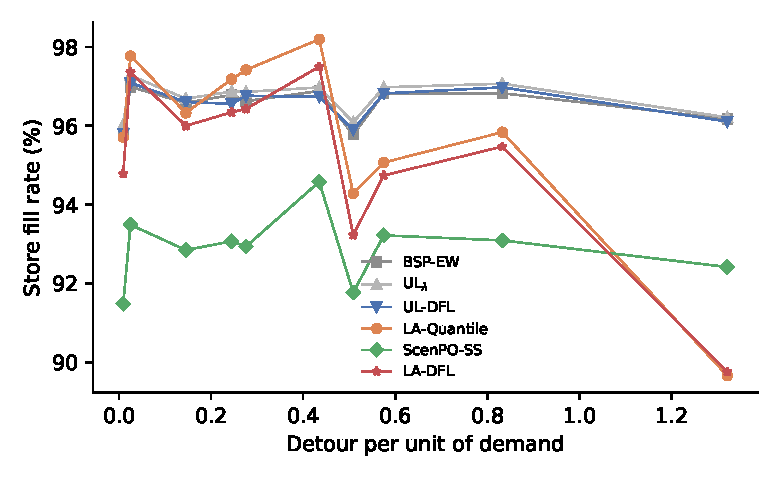
\includegraphics[width=0.6\textwidth]{fig_store_service.pdf}
\caption{Store fill rate against distance from the depot (base case, mean over 100 test episodes).}\label{fig:stores}
\end{figure}

\subsection{Computation}\label{sec:computation}

All \ndecisionsBase{} lookahead decisions of the base-case test were solved to a proven gap of at most \maxgapBase\%, with \nonoptBase{} time-limit stops and \fallbacksBase{} fallbacks; the same holds in every configuration reported. With 15 decisions solved in parallel, a deterministic lookahead decision takes about \secsLAQBase{} seconds and a ScenPO-SS decision \secsScenPOBase{} seconds; the rules, with or without learned corrections, need milliseconds. Training one UL-DFL network (30 epochs over 200 episodes, including closed-loop validation after every epoch) took about two minutes; training one LA-DFL network (2,100 states, eight epochs including MILP re-solves and closed-loop validation) about 45 minutes. The complete base case, including tuning of all policies and three seeds of each learner, took 4.2 hours, and each other configuration 1.0--2.6 hours with 13--15 parallel workers (training three NN-DFL networks adds about ten minutes).

The lookahead policies are deterministic: solving the same decision twice returns the same plan. Their closed-loop cost is nevertheless sensitive to negligible changes in the planning input, because several plans lie within the 0.5\% optimality gap and the solver returns the first one it proves; a different plan on one day changes the stock and therefore every later decision. To quantify this noise floor we re-ran LA-Quantile on the test episodes with its planning targets rounded to single precision, a relative change below $10^{-7}$. The plan changed on at least one day in each of the \noiseN{} test episodes of the thirteen configurations, and episode costs moved by \noiseSDBase\% (standard deviation) in the base case, between \noiseMinBase\% and \noiseMaxBase\%, and by \noiseSDLo--\noiseSDHi\% across configurations. Averaged over 100 episodes these changes largely cancel (mean change at most \noiseAbsMeanMax\% in absolute value, standard error at most \noiseSEHi\%). Paired comparisons remain valid, because this variation is part of the episode-level noise they account for, but differences of well below one percent between two lookahead policies should not be interpreted as a systematic effect. The rule-based policies, including UL-DFL, do not solve an optimisation model for their orders and are not affected.

\subsection{Verification of the structural results}\label{sec:verification}

Table~\ref{tab:verification} reports numerical checks of the results in Section~\ref{sec:theory} (script \texttt{verify\_theory.py} in the replication package). Theorem~\ref{thm:fifo}(ii) is checked by solving the recourse a second time with FIFO issuing and greedy service imposed through binary indicator constraints: if the theorem were false, the constrained value would exceed $V_{\mathrm{LP}}$ in some instance. The bound of Proposition~\ref{prop:marginal}(b) is attained in 71\% of the random instances, so it cannot be tightened in general. The physical FIFO cost equals $V_{\mathrm{LP}}$ in 63\% of the random instances; the remaining gap is the value of discarding stock early, which a store does not do in practice.

\begin{table}[H]
\centering\small
\caption{Numerical verification of the structural results.}\label{tab:verification}
\begin{tabular}{p{3.2cm}p{6.6cm}p{4.0cm}}
\toprule
Result & Check & Outcome \\
\midrule
Theorem~\ref{thm:fifo}(i) & 60 lookahead MILPs ($m\in\{2,3,4\}$, 1 or 5 scenarios) with demand from zero to four times fleet capacity & all feasible, all solved to proven gap \\
Theorem~\ref{thm:fifo}(ii) & 3,000 random recourse instances ($m\in\{2,3,4\}$, $H\in\{2,\dots,5\}$, random costs); FIFO- and greedy-constrained MILP value vs.\ $V_{\mathrm{LP}}$ & max.\ absolute difference $10^{-6}$ \\
Theorem~\ref{thm:fifo}(iii) & $V_{\mathrm{LP}}\le C_{\mathrm{FIFO}}$ in the same instances & holds in 3,000/3,000; equality in 63\% \\
Proposition~\ref{prop:marginal}(a) & dual bounds $[-p_u,p_s]$; subgradient inequality in 9,000 random directions & 3,000/3,000; 9,000/9,000 \\
Proposition~\ref{prop:marginal}(b) & autograd derivative of $C_{\mathrm{FIFO}}$ within \eqref{eq:marg} & 3,000/3,000; bound attained in 71\% \\
Proposition~\ref{prop:dfl}(c) & $m=1$, negative-binomial demand (mean 15), SGD on the decision-focused loss (with $m=1$ both learners deliver the learned quantity, so the check covers (a) and (b)) & learned target 20.03; empirical 0.8-quantile 20.0; $F(\tilde d)=0.809$ vs.\ $p_u/(p_u+p_s)=0.8$ \\
Coverage layer & 40 lookahead MILPs; deliveries implied by the visit pattern vs.\ MILP deliveries & 98.7\% of delivered volume reproduced (mean relative $L_1$ deviation 1.3\%) \\
\bottomrule
\end{tabular}
\end{table}

